% \begin{figure}[htbp]
%     \centering
%     \begin{subfigure}[b]{1\columnwidth}
%         \centering
%         \includegraphics[width=\textwidth]{figs/blackbird_trajs/clover.pdf}
%     \end{subfigure}

%      \vspace{0.1em}
%          \centering
%     \begin{subfigure}[b]{1\columnwidth}
%         \centering
%         \includegraphics[width=\textwidth]{figs/blackbird_trajs/egg.pdf}
%     \end{subfigure}

%      \vspace{0.1em}
%          \centering
%     \begin{subfigure}[b]{1\columnwidth}
%         \centering
%         \includegraphics[width=\textwidth]{figs/blackbird_trajs/winter.pdf}
%     \end{subfigure}
%      \vspace{0.1em}
%          \centering
%     \begin{subfigure}[b]{1\columnwidth}
%         \centering
%         \includegraphics[width=\textwidth]{figs/blackbird_trajs/star.pdf}
%         \caption{SEEN Sequences. From top to bottom: \texttt{Clover}, \texttt{Egg}, \texttt{Winter} and \texttt{Star} sequence. Our method demonstrates robust performance without requiring any additional sensor information.}
%         \label{fig:sub_bb_2}
%     \end{subfigure}

%     \vspace{1em}
%              \centering
%     \begin{subfigure}[b]{1\columnwidth}
%         \centering
%         \includegraphics[width=\textwidth]{figs/blackbird_trajs/bentDice.pdf}
%     \end{subfigure}
%      \vspace{0.1em}
%     \begin{subfigure}[b]{1\columnwidth}
%         \centering
%         \includegraphics[width=\textwidth]{figs/blackbird_trajs/oval.pdf}
%     \end{subfigure}

%      \vspace{0.1em}
%          \centering
%     \begin{subfigure}[b]{1\columnwidth}
%         \centering
%         \includegraphics[width=\textwidth]{figs/blackbird_trajs/sphinx.pdf}
%         \caption{UNSEEN Sequences. From top to bottom: \texttt{bentDice}, \texttt{Oval}, and \texttt{Sphinx} sequence. Our method demonstrates remarkable adaptability to trajectories it has never seen before.}
%         \label{fig:sub_bb_1}
%     \end{subfigure}
%     \caption{Estimated trajectories of Blackbird dataset by RoNIN, TLIO, IMO and AirIO (Ours). }
%     \label{fig:blackbird-trajs}
% \end{figure}

\begin{figure}[h]
    \centering
    \includegraphics[width=0.8\columnwidth]{tex/ch6_airio/figs/blackbird_trajs/clover.pdf}
    \vspace{0.1em}
    \includegraphics[width=0.8\columnwidth]{tex/ch6_airio/figs/blackbird_trajs/egg.pdf}
    \vspace{0.1em}
    \includegraphics[width=0.8\columnwidth]{tex/ch6_airio/figs/blackbird_trajs/winter.pdf}
    \vspace{0.1em}
    \includegraphics[width=0.8\columnwidth]{tex/ch6_airio/figs/blackbird_trajs/star.pdf}
    \caption{SEEN Sequences. From top to bottom: \texttt{Clover}, \texttt{Egg}, \texttt{Winter} and \texttt{Star}. Our method demonstrates robust performance without requiring any additional sensor information.}
    \label{fig:airio:bb_seen}
\end{figure}

\begin{figure}[h]
    \centering
    \includegraphics[width=0.8\columnwidth]{tex/ch6_airio/figs/blackbird_trajs/bentDice.pdf}
    \vspace{0.1em}
    \includegraphics[width=0.8\columnwidth]{tex/ch6_airio/figs/blackbird_trajs/oval.pdf}
    \vspace{0.1em}
    \includegraphics[width=0.8\columnwidth]{tex/ch6_airio/figs/blackbird_trajs/sphinx.pdf}
    \caption{UNSEEN Sequences. From top to bottom: \texttt{bentDice}, \texttt{Oval}, and \texttt{Sphinx}. Our method demonstrates remarkable adaptability to trajectories it has never seen before.}
    \label{fig:airio:bb_unseen}
\end{figure}
